\section{Data}
\label{sec:data}
In order to perform the experimentation and to compare both clustering algorithms, we created different scenarios using the module \code{dataset} of the \textit{scikit-kearn} \cite{scikit-learn} package of Python. These scenarios consist in 2-D points located in different places among the space, forming clusters of different shapes (blob, circle and moon). They are shown in figure \ref{fig:truth-data}. 

We also used the dataset of the previous work (Data mining techniques applied to medicine), which is the Heart Disease dataset \cite{heart}, to see how the algorithms behave with realistic data.

\begin{figure}[hbtp]
    \begin{subfigure}[b]{0.45\columnwidth}
        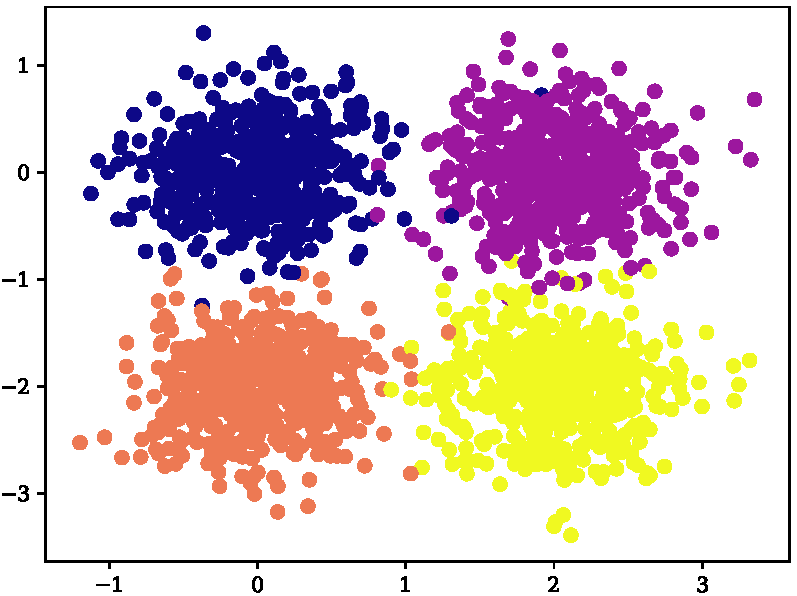
\includegraphics[width=\columnwidth]{../plots/truth_4-4.pdf}
        \caption{4 blobs}
        \label{subfig:4-4-truth}
    \end{subfigure}
    \hspace{0.04\columnwidth}
    \begin{subfigure}[b]{0.45\columnwidth}
        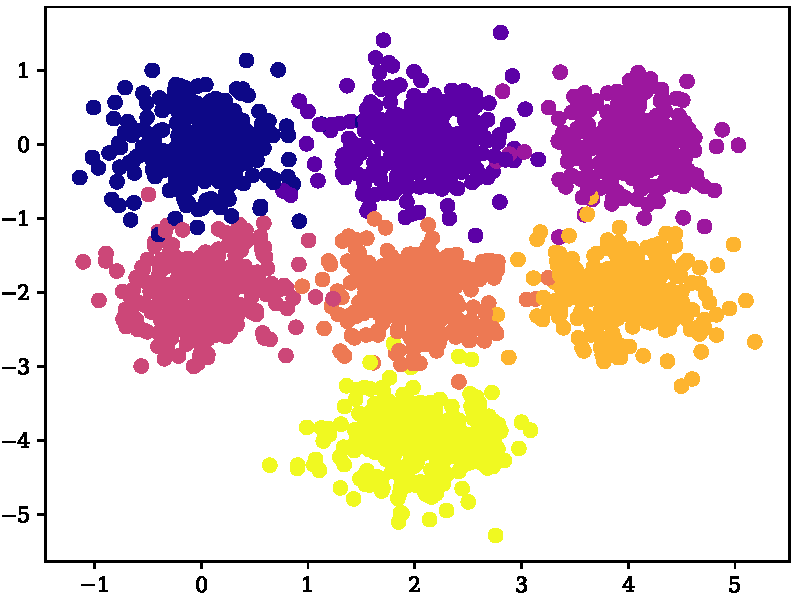
\includegraphics[width=\columnwidth]{../plots/truth_7-3.pdf}
        \caption{7 blobs}
        \label{subfig:7-3-truth}
    \end{subfigure}
    \begin{subfigure}[b]{0.45\columnwidth}
        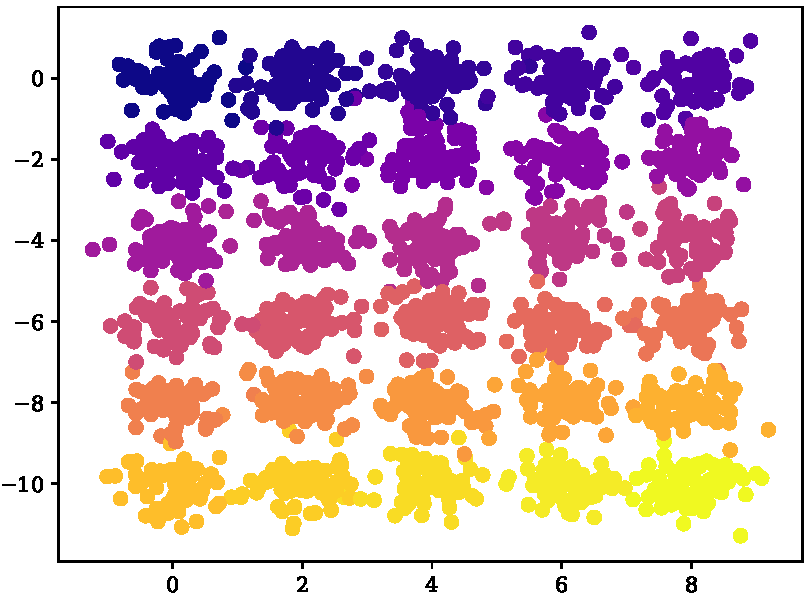
\includegraphics[width=\columnwidth]{../plots/truth_30-30.pdf}
        \caption{30 blobs}
        \label{subfig:30-30-truth}
    \end{subfigure}
    \hspace{0.04\columnwidth}
    \begin{subfigure}[b]{0.45\columnwidth}
        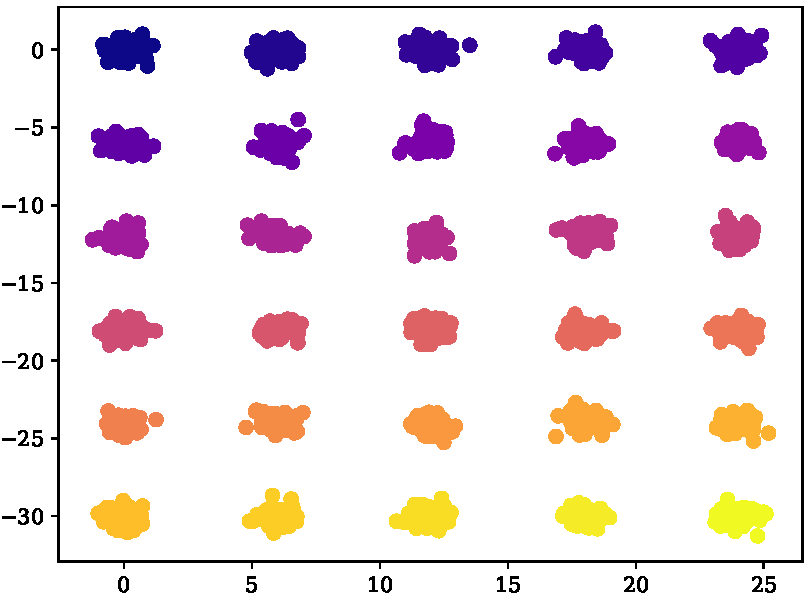
\includegraphics[width=\columnwidth]{../plots/truth_30-30-6.pdf}
        \caption{30 spaced blobs}
        \label{subfig:30-30-6-truth}
    \end{subfigure}
    \begin{subfigure}[b]{0.45\columnwidth}
        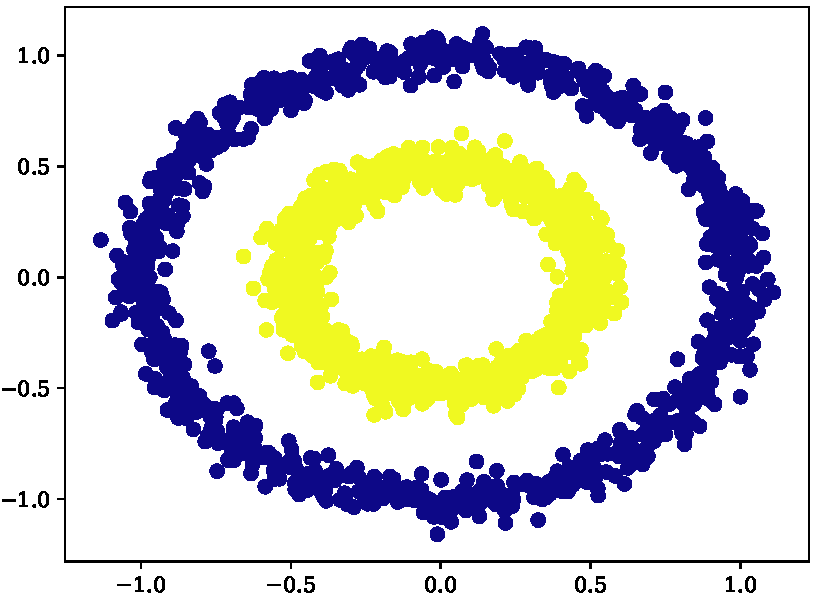
\includegraphics[width=\columnwidth]{../plots/circle_dbscan.pdf}
        \caption{2 circles}
        \label{subfig:circle-truth}
    \end{subfigure}
    \hspace{0.04\columnwidth}
    \begin{subfigure}[b]{0.45\columnwidth}
        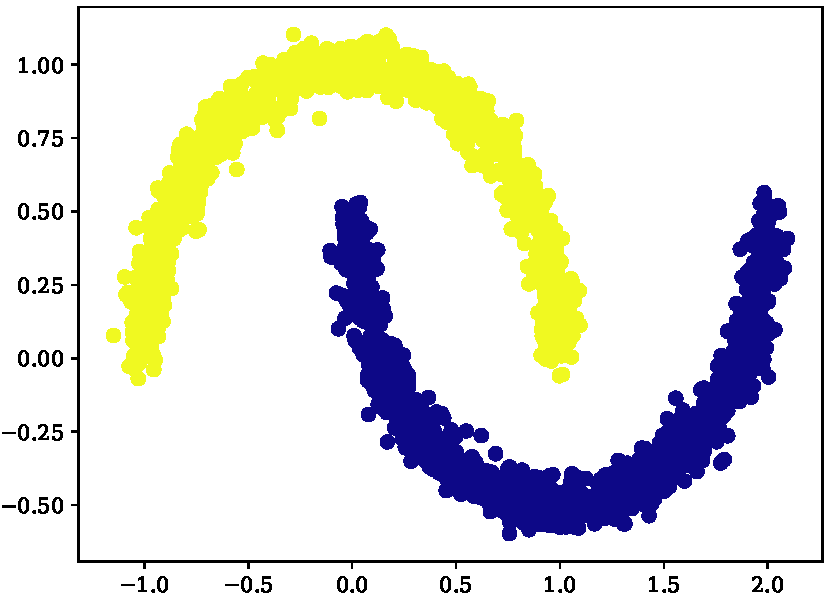
\includegraphics[width=\columnwidth]{../plots/moons_dbscan.pdf}
        \caption{2 moons}
        \label{subfig:moons-truth}
    \end{subfigure}
    \caption{Generated data}
    \label{fig:truth-data}
\end{figure}

%We explain how we created them in section \ref{sec:experimentation}.